%%%%%%%%%%%%%%%%%%%%%%%%%%%%%%%%%%%%%%%%%%%%%%%%%%%%%%%%%%%%%%%%%%%%%%%%%%%%%%%%
%2345678901234567890123456789012345678901234567890123456789012345678901234567890
%        1         2         3         4         5         6         7         8

\documentclass[letterpaper, 10 pt, conference]{ieeeconf}
\usepackage{blindtext, graphicx}
\usepackage{pgfplots}
\usepackage{xcolor}
\usepackage{tikz}
\usepackage{lipsum,adjustbox}
\usepackage{listings}
\usepackage{fancyhdr}

% Comment this line out if you need a4paper

%\documentclass[a4paper, 10pt, conference]{ieeeconf}      % Use this line for a4 paper

\IEEEoverridecommandlockouts                              % This command is only needed if 
                                                          % you want to use the \thanks command

\overrideIEEEmargins                                      % Needed to meet printer requirements.

% See the \addtolength command later in the file to balance the column lengths
% on the last page of the document

% The following packages can be found on http:\\www.ctan.org
%\usepackage{graphics} % for pdf, bitmapped graphics files
%\usepackage{epsfig} % for postscript graphics files
%\usepackage{mathptmx} % assumes new font selection scheme installed
%\usepackage{times} % assumes new font selection scheme installed
%\usepackage{amsmath} % assumes amsmath package installed
%\usepackage{amssymb}  % assumes amsmath package installed

\title{\LARGE \bf
ECE 590 HW4: Scalability
}


\author{Nisarg Dabhi and Connor Grehlinger} 


\begin{document}



\maketitle
\thispagestyle{empty}
\pagestyle{empty}


%%%%%%%%%%%%%%%%%%%%%%%%%%%%%%%%%%%%%%%%%%%%%%%%%%%%%%%%%%%%%%%%%%%%%%%%%%%%%%%%
\begin{abstract}

This document serves as a performance and scalability analysis of an Exchange Matching Server developed for Homework 4 of ECE590 Engineering Robust Server Software

\end{abstract}

%%%%%%%%%%%%%%%%%%%%%%%%%%%%%%%%%%%%%%%%%%%%%%%%%%%%%%%%%%%%%%%%%%%%%%%%%%%%%%%%
\section{Testing Scalability of Underlying Exchange Server Infrastructure}

The TCP server our Exchange Matching server runs on is a subclass of the Poco library’s Poco::Net::TCPServer. This is a multi-threaded TCP server which uses a thread pool and dispatches threads from that pool to handle connections to the server. One thread is responsible for listening for incoming connections on a queue, then accepting those connections and dispatching other threads to handle connection interaction with the client end host.
 
 
 
Our exchange server allows a maximum connection queue of 8192 connections. Threads waiting to accept connections which are idle for more than 10 seconds are terminated. These parameters can be adjusted to accommodate the Exchange Server’s load.



The VM on which the Exchange Matching Server runs has the following specifications: 


\begin{figure}[!htb]
    \centering
    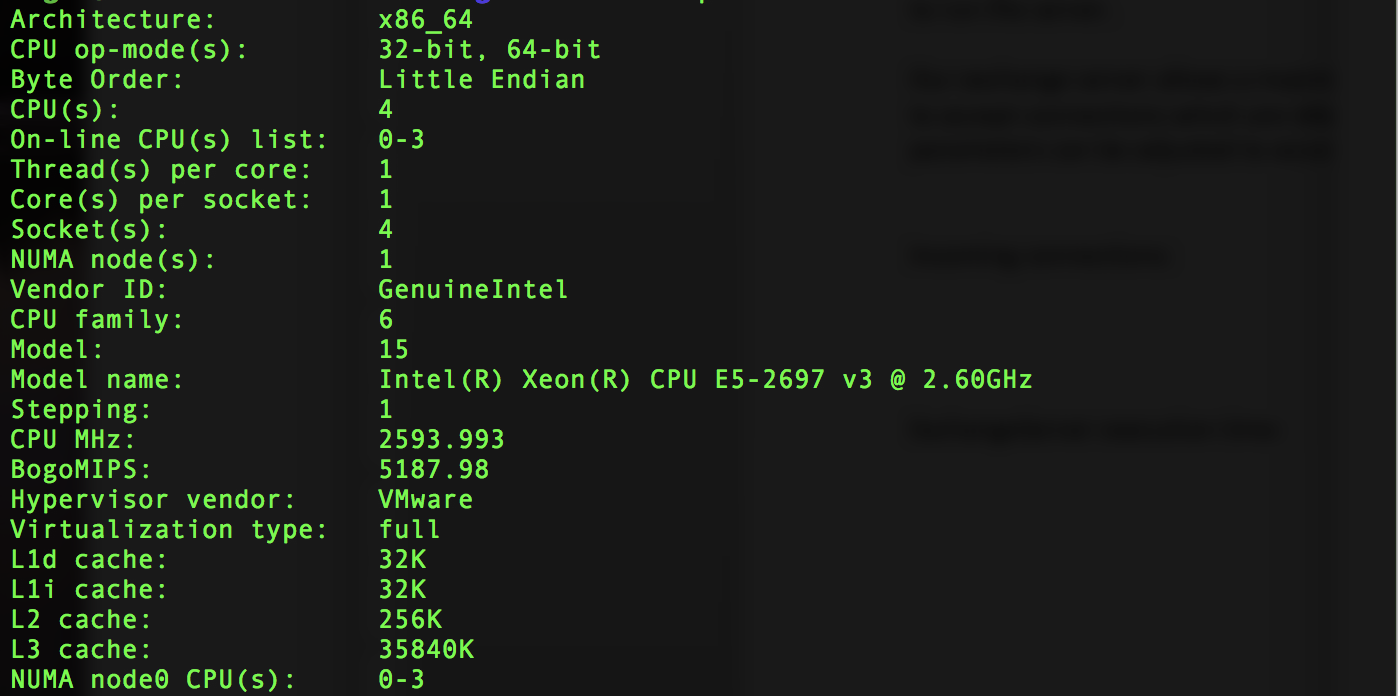
\includegraphics[height=3.8cm, width=7.8cm]{ExchangeVm.png}
    \caption{Exchange Matching Server VM 
    Specifications}
    \label{fig:Exchange}
\end{figure}


\begin{figure}[!htb]
    \centering
    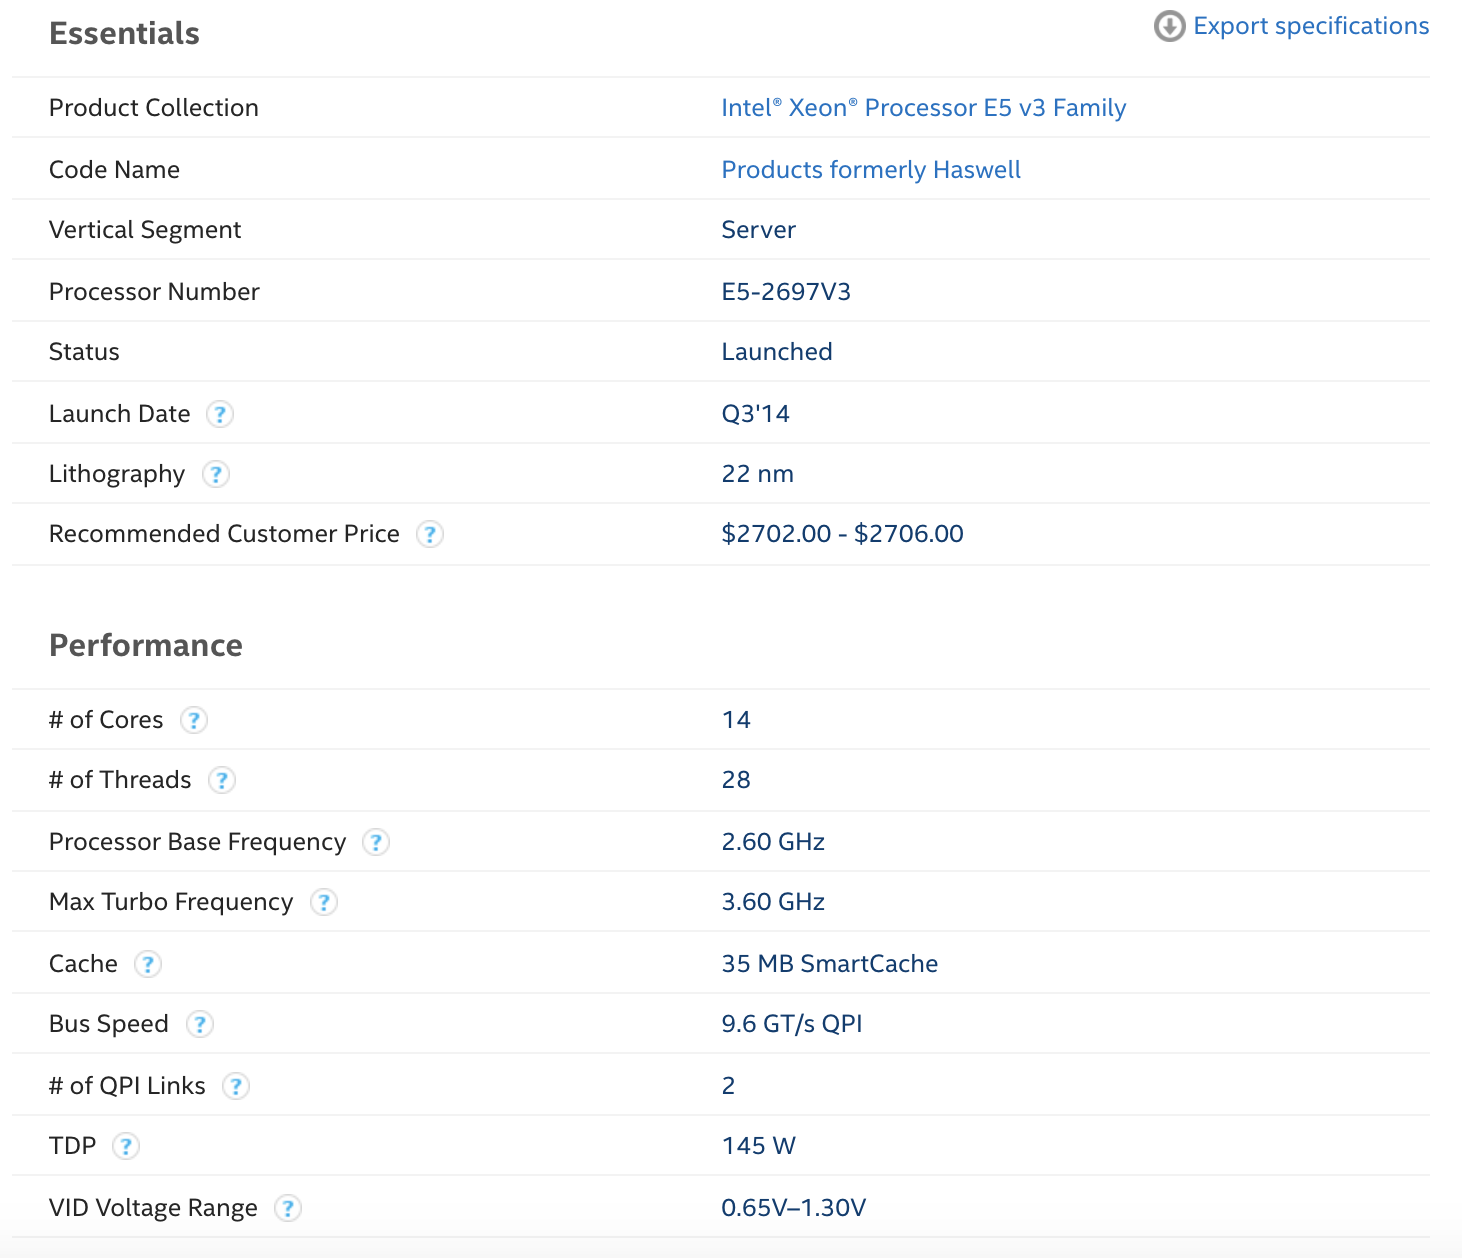
\includegraphics[height=7cm, width=7.7cm]{ExchangeCPU.png}
    \caption{Exchange Matching Server
    VM Intel CPU Specifications}
    \label{fig:Intel}
\end{figure}

This VM uses a portion of the resources of the Intel CPU listed. Specifications for this particular Intel chip are depicted in Figure \ref{fig:Intel}. It is clear that the physical chip itself has more resources than what is allocated to the VM:

Since this is an Intel chip which supports hyper threading, based on what our virtual machine has been allocated we have 8 hardware threads:
 
2 threads/core * 1 core/socket * 4 sockets = 8 threads
 
The graphics on the next page depict the scalability of the underlying multi-threaded TCP Server our Exchange Matching Server uses. These figures represent the performance of basic TCP connections and transmissions. The Exchange Matching Server receives an example string of XML (see Figure \ref{fig:XML}) and responds to the client by sending the message “Request received by exchange server”.
 
 \begin{figure}[!htb]
    \centering
    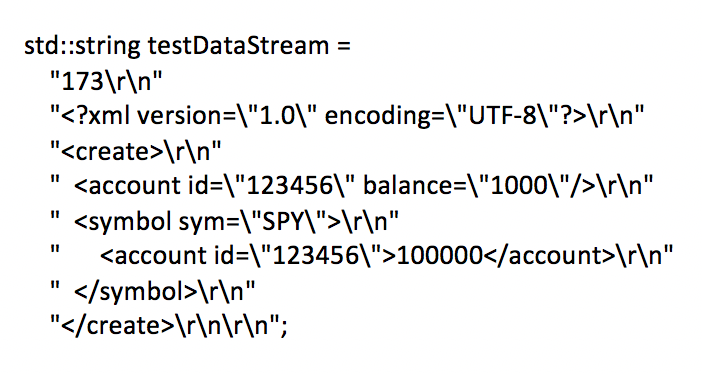
\includegraphics[height=3.8cm, width=7.8cm]{XMLExmaple.png}
    \caption{Example XML string}
    \label{fig:XML}
\end{figure}
 
 
\section{Connection \& Transmission Stress Test}


 \begin{figure}[!htb]
    \centering
    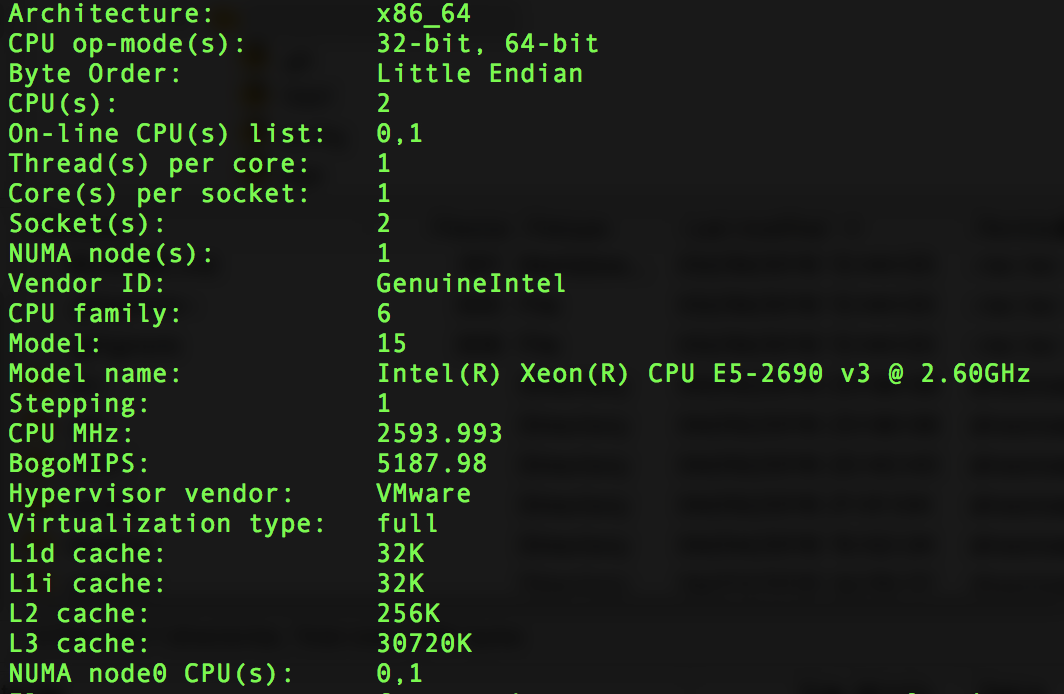
\includegraphics[height=3.8cm, width=7.8cm]{TesterVm.png}
    \caption{Separate VM Specifications}
    \label{fig:NewVM}
\end{figure}

Incoming connections: Incoming connection requests and XML string transmission are made by a VM separate from the Exchange Matching server with the specifications shown in Figure ~\ref{fig:NewVM}.



A test program on this machine uses a thread 
pool to dispatch threads to make a new 
connection and send the XML string then receive a reply. 



The number of threads dispatched to send 
requests as well as the number of 
requests each thread sends can be 
tuned with parameters \texttt{THREADS} and 
\texttt{REQUESTS}. The thread pool is set to a 
min size equal to the \texttt{THREADS} parameter and max size of 2048.



NOTE: The max thread capacity for the thread 
pools on both the Exchange Matching Server and 
the VM which is load testing are set to 4096 
and 2048 respectively. This is far higher than 
either machine can support, but this to ensure 
each machine uses as much execution resources 
as possible for the scalability stress test)



Instructions for using our testing suite as are written below. They can also be found in the 
README.md file of the /testing/ directory of 
the repository: 
  
\section{Testing Exchange Server Scalability}  



To run performance tests measuring scalability 
in the context of execution time under certain 
request volumes, make changes to the 
following macro fields:
\begin{itemize}
  \item \textbf{{REQ} in 
    /src/ExchangeRequestHandler.cpp}
\end{itemize}
   

   
   This sets the number of requests the
   Exchange Matching Server will handle before
   terminating and printing the execution time
   it took to process those requests in
   microseconds and seconds. The total running
   time of the Exchange Server Application is
   also reported.
     
\begin{itemize}
\item \textbf{THREADS in /testing/src/XMLRequestGen.cpp}
\end{itemize}

 This sets the number of threads which will be
 dispatched from a thread pool to perform a number of iterations (defined by the REQUESTS macro) of a function (called runTest) which load tests the Exchange Matching Server. In each iteration of the load testing function:
 
 
 
\begin{enumerate}
\item A new connection is established with the Exchange Matching Server
\item A request containing an XML string is sent to the Exchange Matching Server
\item A reply sent by the Exchange Matching Server is received by the calling thread
\end{enumerate}

\begin{itemize}
\item \textbf{REQUESTS in /testing/src/XMLRequestGen.cpp}
\end{itemize}
 
 
 
This specifies the number of iterations of the 
load testing function (runTest) each thread
completes.This means THREADS * REQUESTS is the
total number of connect + send + receive calls 
made to the Exchange Matching Server on each call to ./XMLRequestGen.




\begin{itemize}
\item \textbf{The docker-compose.yml file in /testing/}
\end{itemize}
Ensures that the bash command on line 6
iterates through and calls the ./XMLRequestGen
program enough times to generate enough
requests to hit the REQ macro threshold
in /src/ExchangeRequestHandler.cpp:
    
    
   
   \[ (XMLRequestGen calls * THREADS 
   *REQUESTS)
   \geq (REQ)  
    \] 
    


\subsection{Scalability Testing Results}

\begin{figure}[!htb]
    \centering
    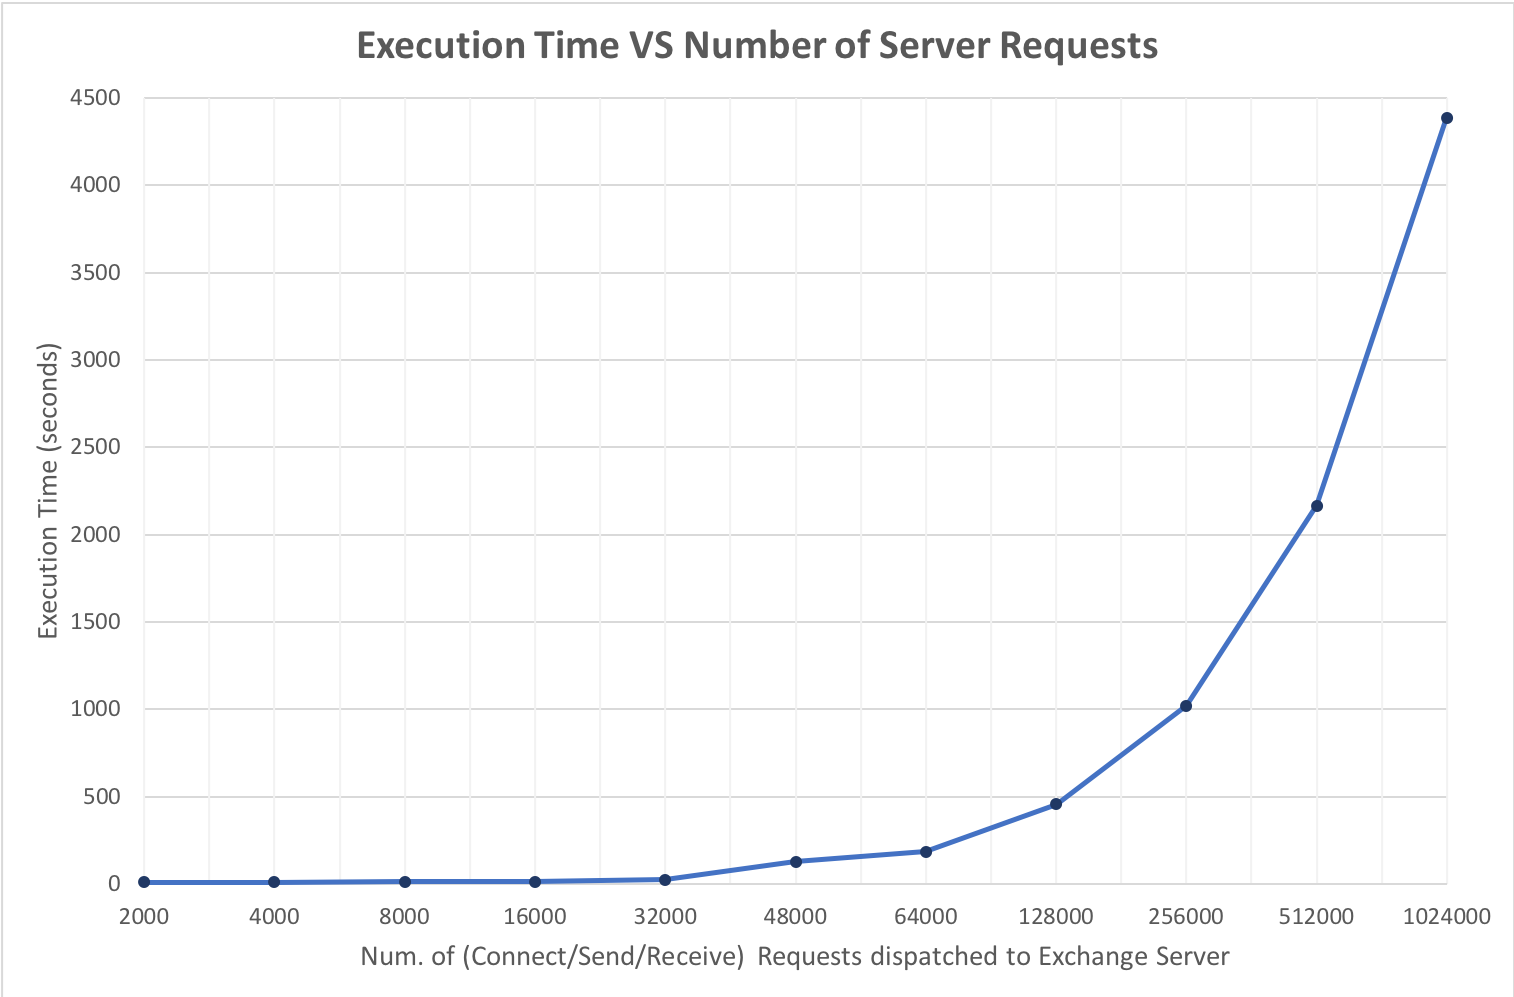
\includegraphics[height=5.5cm, width=8.6cm]{exeTime_v_numReqs.png}
    \label{fig:my_label}
\end{figure}


\begin{figure}[!htb]
    \centering
    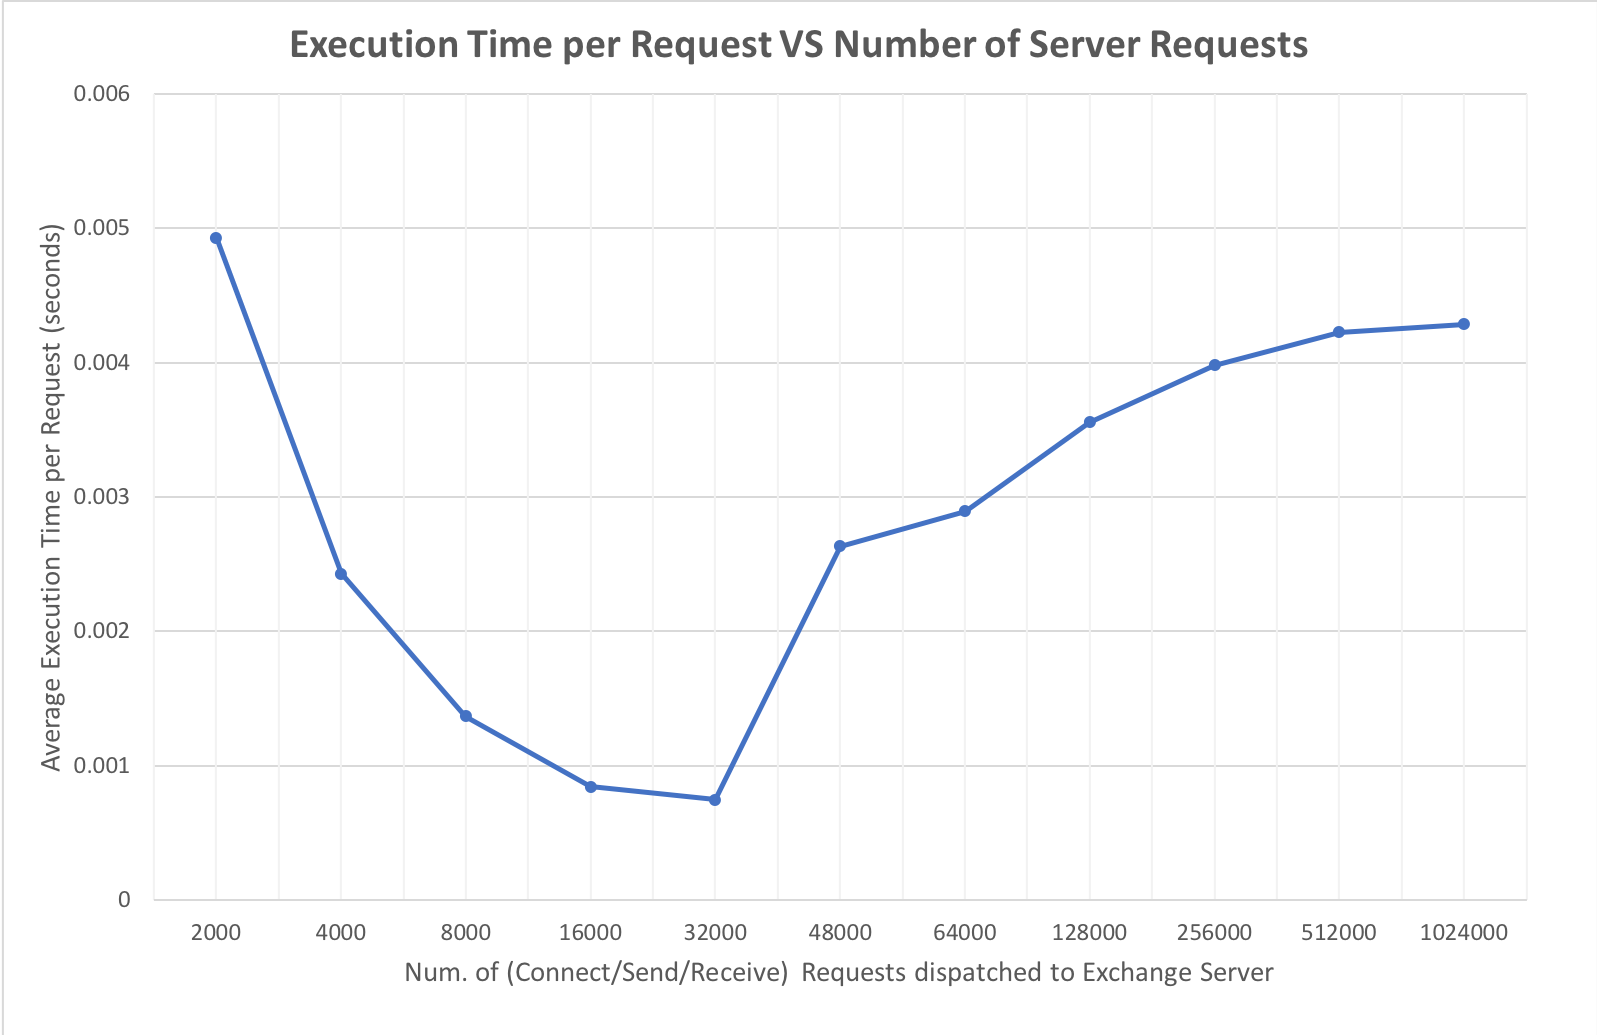
\includegraphics[height=5.5cm, width=8.6cm]{exeTime_perReq_v_numReq.png}
    \label{fig:my_label}
\end{figure}

From both depicted graphs it is clear that the underlying TCP Server for
our Exchange Matching Server is scalable within the limitations of the 
provided hardware.

The Execution Time vs Number of Requests dispatched to the server graph
(each request established a connection, sends a message, and receives a
reply) shows a near linear relationship. Each time the number of
dispatched requests doubles the execution time to complete those requests
also about doubles.

The Execution Time per Request vs Number of Requests graph also shows
little variably in the servicing time of each request even if the load on
the Exchange Matching Server is greatly increased. What little 
variability which can be seen is measured in milliseconds and can be 
attributed to variability in transmissions over TCP networks. 

The table which was used to calculate these results is included below:
% 
% \being{figure}[!htb]
    % \centering
    % 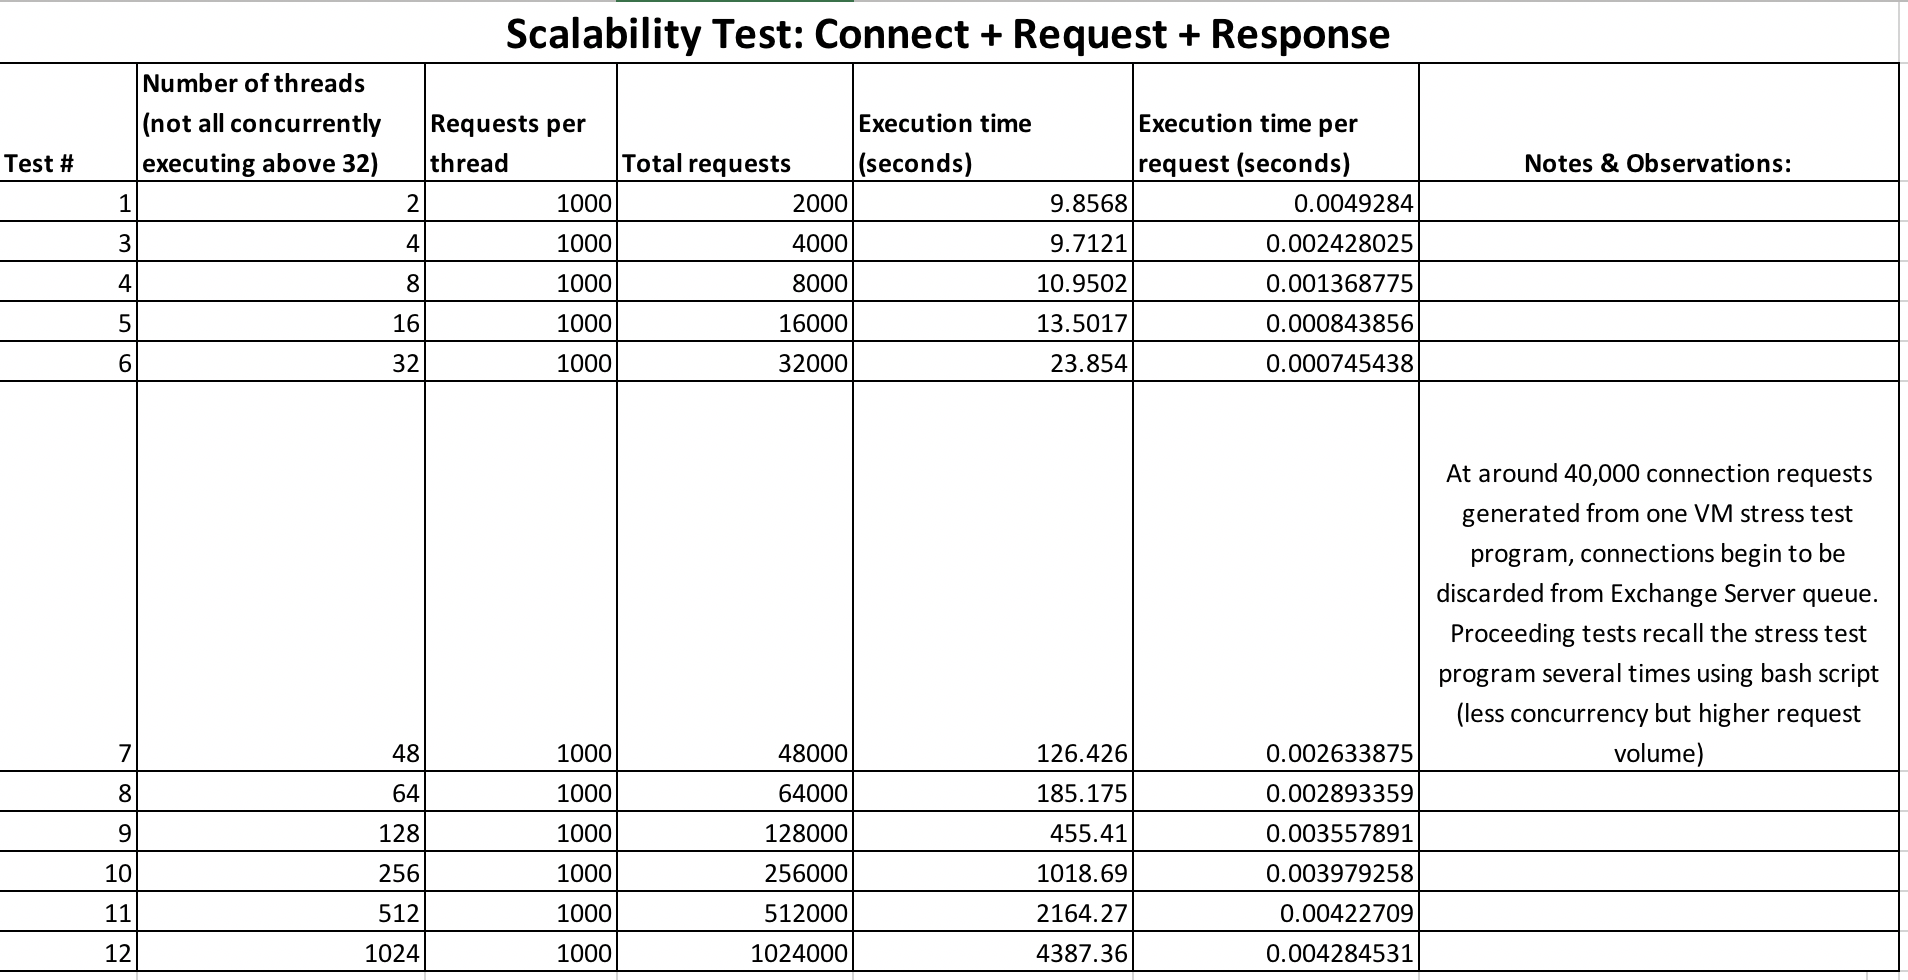
\includegraphics[height=5.5cm, width=8.6cm]{Scalability_test_table.png}
    % \label{fig:my_label}
% \end{figure}

\begin{figure}[!htb]
   \centering
    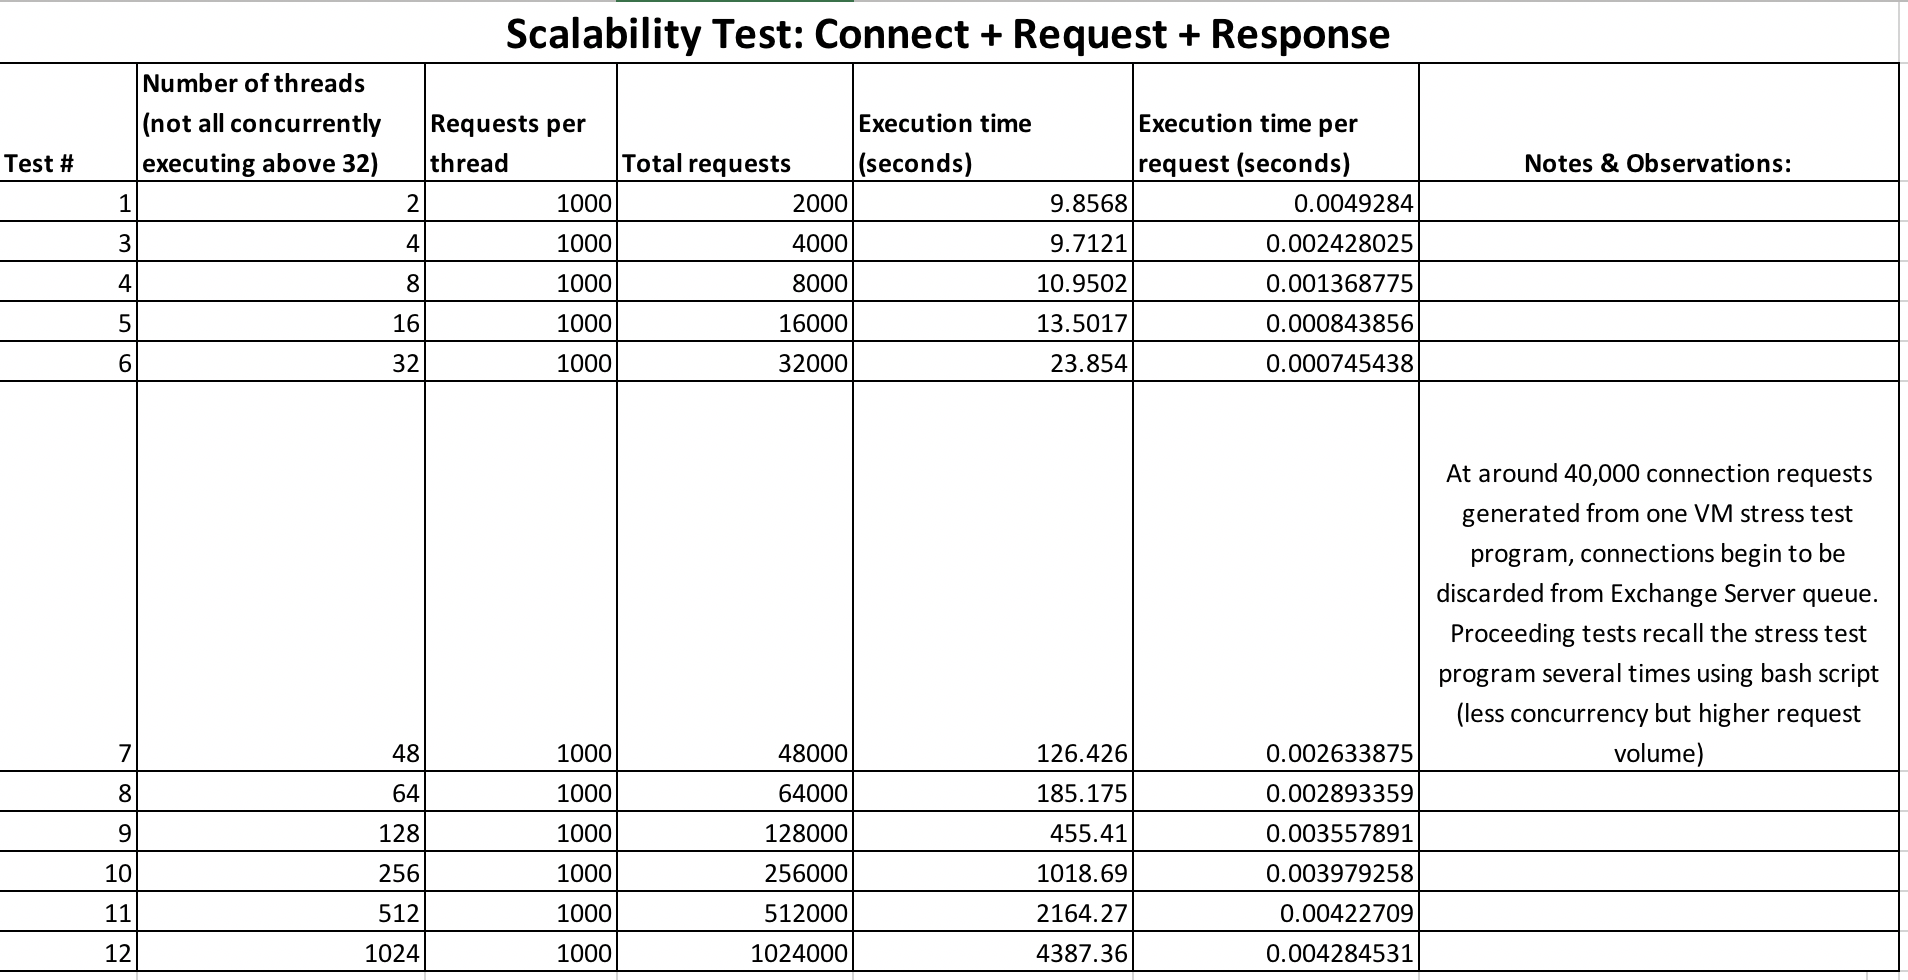
\includegraphics[height=10.5cm, width=18.6cm]{Scalability_test_table.png}
    \label{fig:my_label}
\end{figure}




\end{document}
